\documentclass[12pt]{report}

\usepackage{setspace}
\setlength{\parindent}{4em}

\usepackage{fancyvrb}
\usepackage{graphicx}
\usepackage{geometry}

\geometry{letterpaper, portrait, margin=1in}

%%%Title Page%%%
\title{
  Lab 08
\bigbreak Binary to Binary Coded Decimal
}

\author{
{\normalsize
\begin{tabular}{l r r}
 & \textbf{Ryan Cruz} & \textbf{Zachary Davis}\\
\textbf{Category} & ryan.cruz25@uga.edu & zachdav@uga.edu\\
\hline
Pre-lab 						  & 50 & 50\\
In-lab Module \& Testbench Design & 50 & 50\\
In-lab Testbench Sim. \& Analysis & 50 & 50\\
In-lab FPGA Synthesis \& Analysis & 50 & 50\\
Lab Report Writing 				  & 50 & 50\\
\end{tabular}
}
}

\date{\bigskip
\today}
%%%%%%%%%%%%

\begin{document}
\maketitle

\section*{Lab Purpose}
	\paragraph{}
		The purpose of this lab is to improve the functionality of our previous lab in which we counted and displayed a 4-bit binary number as a hexadecimal number. In this lab, we will improve that design by displaying the 4-bit binary number as a two digit decimal number between \texttt{00} and \texttt{15}. This can be accomplished by designing a Binary to Binary Coded Decimal Converter and a Multiplexed BCD Display Driver to display the output on the two 7-segment displays connected to the Spartan-3E FPGA.
\section*{Implementation Details}
	% \subsection*{Pre-Lab Design}
	% 	\paragraph*{Finite-State-Machine}

	% 		\begin{center}
	% 			%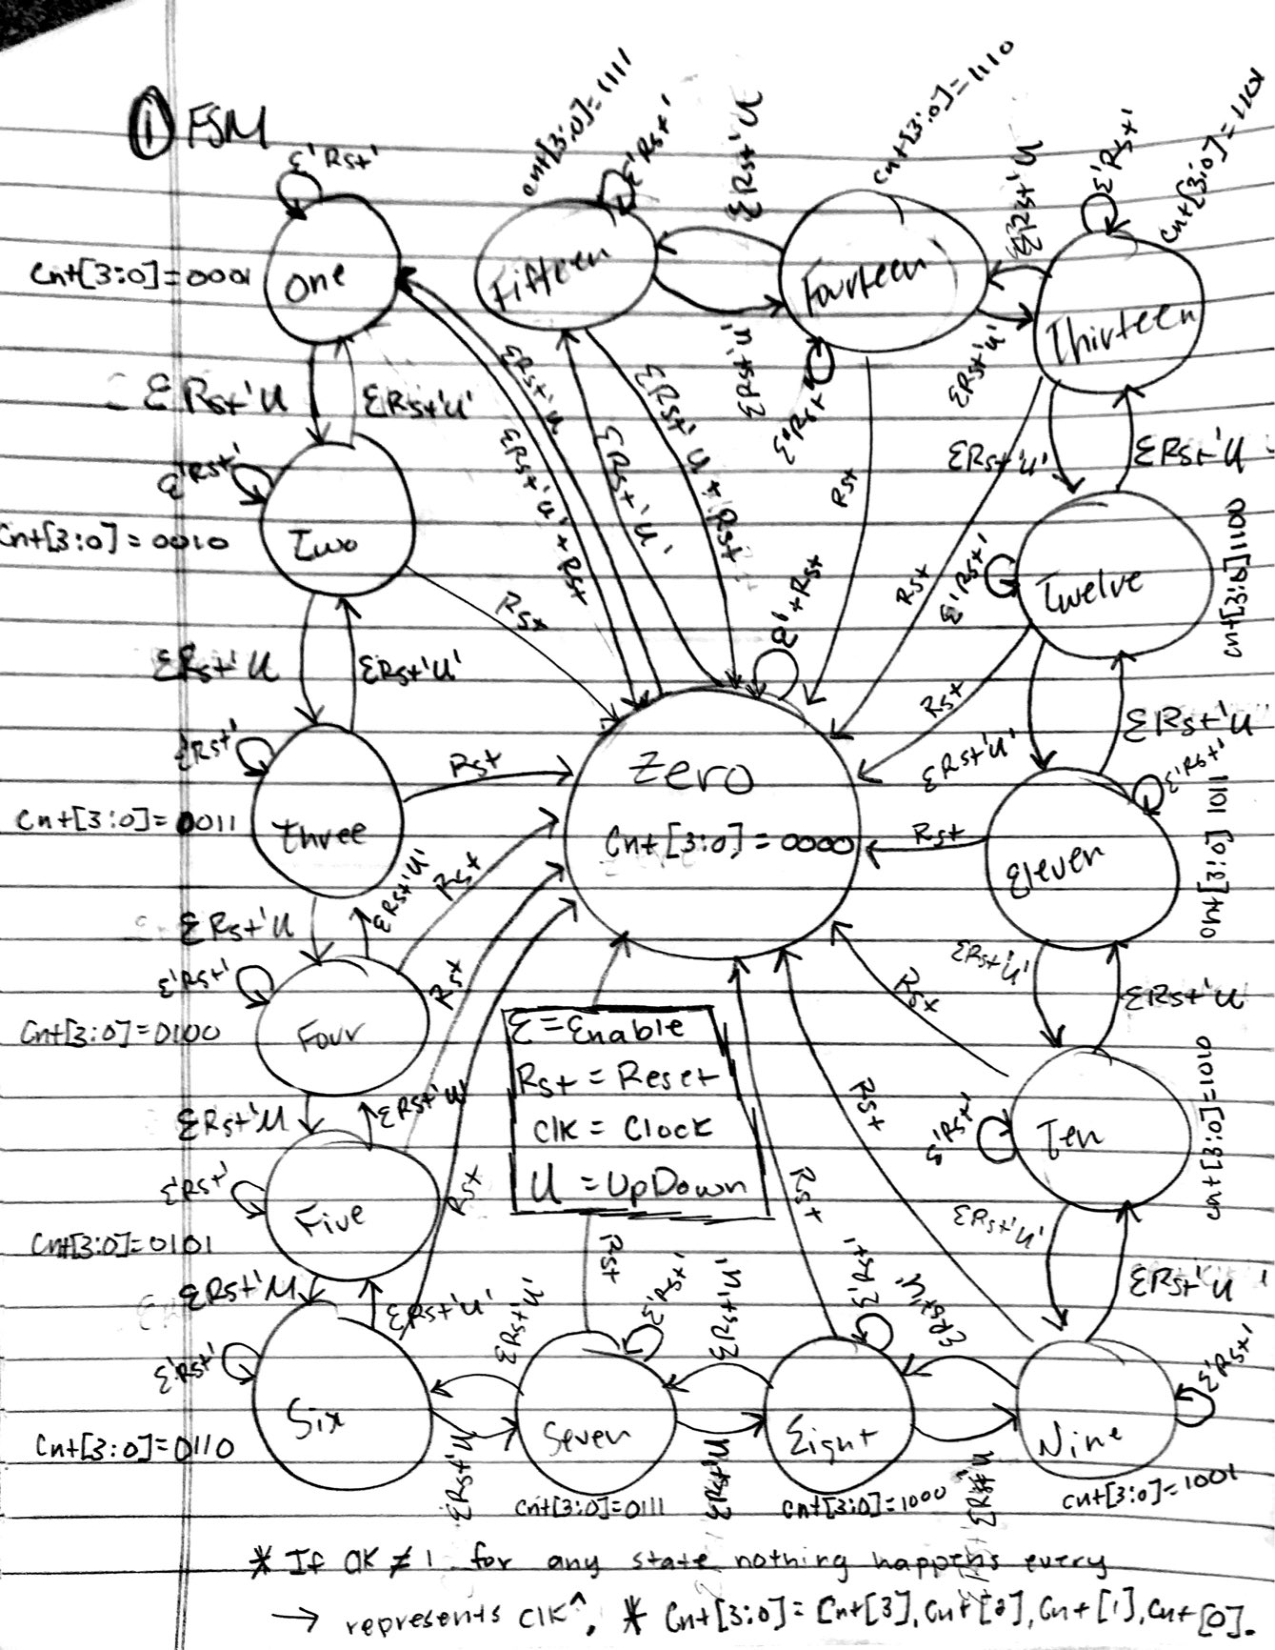
\includegraphics[scale=.5]{Prelab_7-page1.pdf}
	% 		\end{center}

	% 			\paragraph*{}

	% 	\paragraph*{Controller Design}

	% 		\begin{center}
	% 			%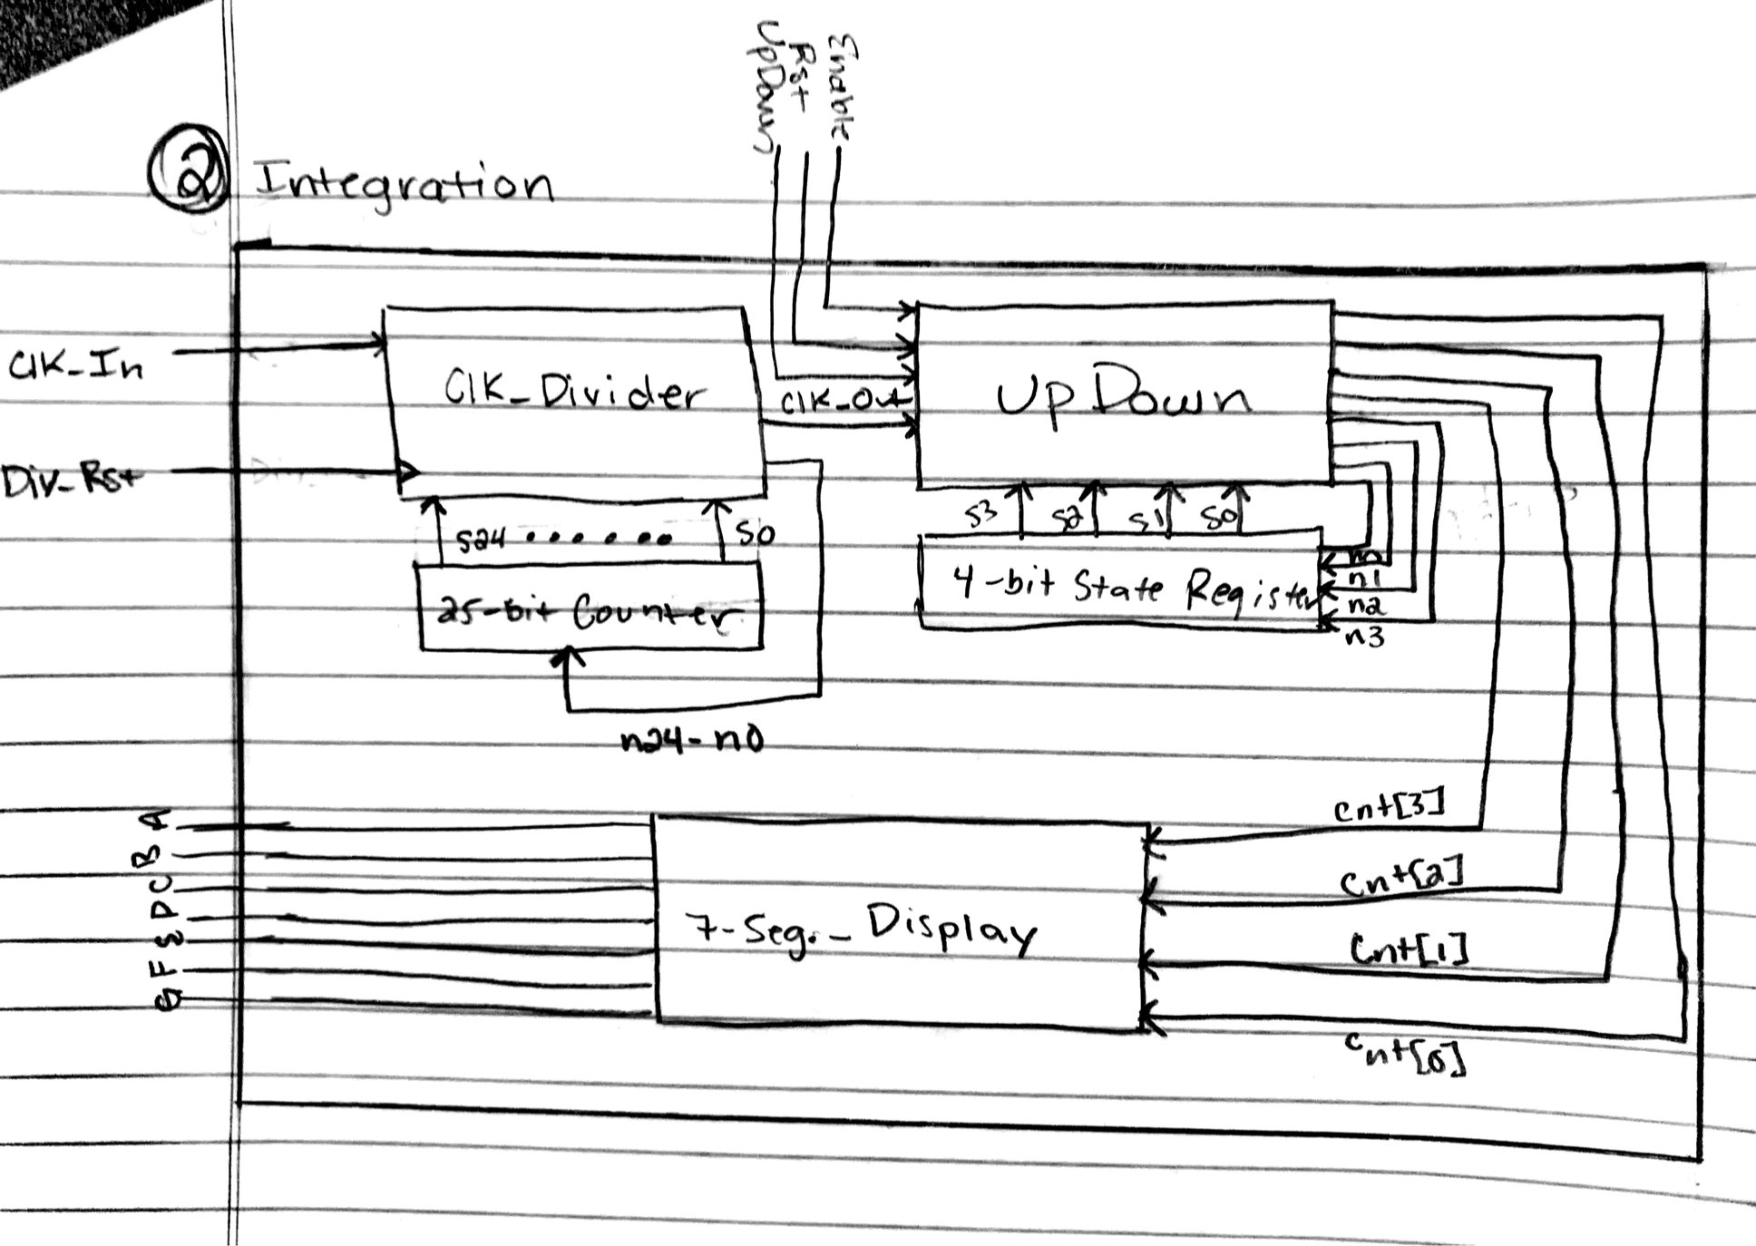
\includegraphics[scale=.5]{Prelab_7-page2.pdf}
	% 		\end{center}
				
	% 			\paragraph*{}
\subsection*{Display Driver}
		\paragraph*{}
		The purpose of this module is to properly display the UpDown value in Binary Coded Decimal using both seven segment digits.
		\vspace{0.3cm}\\
		\textbf{Test Bench Code}
			\begin{Verbatim}[frame=single, fontsize=\small]
`timescale 1ns / 1ps
////////////////////////////////////////////////////////////////////////////////
// Company:        Zachary Davis & Ryan Cruz
// Engineer: 
// 
// Create Date:    13:43:37 10/30/2017 
// Design Name: 
// Module Name:    
// Project Name:   Binary to Binary Coded Decimal
//
////////////////////////////////////////////////////////////////////////////////
module Display_Driver_tb();
	reg Clk_s, Rst_s;
	reg [3:0] Tens_s;
	reg [3:0] Ones_s;
	wire A_s, B_s, C_s, D_s, E_s, F_s, G_s; 
	wire Refresh_s;
	wire [3:0] DValue_s;
	wire Selector_s;
	
	Refresh Refresh_1 (Clk_s, Rst_s, Refresh_s, Selector_s);
	Mux2x1 Mux2x1_1 (Tens_s, Ones_s, Refresh_s, DValue_s);
	Seven_Segment_Display 
	Seven_Segment_Display_1 (DValue_s, A_s, B_s, C_s, D_s, E_s, F_s, G_s);
		
	always
		begin
			Clk_s <= 1;
			#10;
			Clk_s <= 0;
			#10;
	end
	
	initial 
	begin
		Rst_s <= 1; Tens_s <= 4'b0000; Ones_s <= 4'b0000;
		#20;
		Rst_s<= 0; Tens_s <= 4'b0001; Ones_s <= 4'b0000;
		#50 $display ("DValue_s = %b", DValue_s);
		Rst_s<=0; Tens_s <= 4'b0001; Ones_s <= 4'b0001;
		#50 $display ("DValue_s = %b", DValue_s);
		Rst_s <= 0; Tens_s <= 4'b0001; Ones_s <= 4'b0011;
		#50 $display ("DValue_s = %b", DValue_s);
		Rst_s<=0; Tens_s <= 4'b0001; Ones_s <= 4'b0010;
		#50 $display ("DValue_s = %b", DValue_s);
		Rst_s<=0; Tens_s <= 4'b0000; Ones_s <= 4'b1111;
		#50 $display ("DValue_s = %b", DValue_s);
		Rst_s<=0; Tens_s <= 4'b0000; Ones_s <= 4'b1000;
		#50 $display ("DValue_s = %b", DValue_s);
		Rst_s<=0; Tens_s <= 4'b0000; Ones_s <= 4'b1010;
		#50 $display ("DValue_s = %b", DValue_s);
	end
endmodule
			\end{Verbatim}

		\paragraph*{}

\subsection*{Refresh}
		\paragraph*{}
		The purpose of this code is to refresh the two seven segment displays seperately and update the display seperetly.
		\vspace{0.3cm}\\
		\textbf{Behavioral Module Code}
			\begin{Verbatim}[frame=single, fontsize=\small]
`timescale 1ns / 1ps
////////////////////////////////////////////////////////////////////////////////
// Company:        Zachary Davis & Ryan Cruz
// Engineer: 
// 
// Create Date:    13:43:37 10/30/2017 
// Design Name: 
// Module Name:    Refresh
// Project Name:   Binary to Binary Coded Decimal
//
////////////////////////////////////////////////////////////////////////////////
module Refresh(Clk, Rst, Refresh, Selector);
   input Clk, Rst;
   output reg Refresh, Selector;
  
   parameter Divider = 2;
   reg[19:0] Counter;
   reg Clk_Count;
	
   always @(posedge Clk) begin
      if( Rst == 1 )begin
         Counter <= 0;
         Refresh <= 0;
			Selector <=0;
         Clk_Count <= 0;
      end
      else begin
         if( Counter == Divider ) begin
            Refresh <= ~Clk_Count;
				Selector <= ~Clk_Count;
            Clk_Count <= ~Clk_Count;
            Counter <= 0;
         end
         else begin
            Refresh <= Clk_Count;
				Selector <= Clk_Count;
            Clk_Count <= Clk_Count;
            Counter <= Counter + 1;
         end
      end
   end
endmodule
			\end{Verbatim}

				\paragraph*{}

		
		\flushleft
		\textbf{Test Bench Code}
			\begin{Verbatim}[frame=single, fontsize=\small]
`timescale 1ns / 1ps
////////////////////////////////////////////////////////////////////////////////
// Company:        Zachary Davis & Ryan Cruz
// Engineer: 
// 
// Create Date:    13:43:37 10/30/2017 
// Design Name: 
// Module Name:    Refresh
// Project Name:   Binary to Binary Coded Decimal
//
////////////////////////////////////////////////////////////////////////////////
module Refresh_tb();
	reg Clk_t, DivRst_t;
	wire Refresh_t, Selector_t;
	
	Refresh Refresh_1(Clk_t, DivRst_t, Refresh_t, Selector_t);
	
	always
		begin
			Clk_t <= 1;
			#10;
			Clk_t <= 0;
			#10;
		end
	
	initial 
	begin
		DivRst_t <= 0;
		#100;
		DivRst_t <= 1;
		#200;
		DivRst_t <= 0;
	end
endmodule
			\end{Verbatim}
				
				\paragraph*{}

	\subsection*{Binary to BCD}
		\paragraph*{}
		This is the actual module that coverts the hexidecimal value to binary coded decimal by spliting it up into tens and ones.  When ones reaches 10 it is reset to 0 and tens becomes one.  The opposite occurs when counting down from 10 to 9.
		\vspace{0.3cm}\\
		\textbf{Behavioral Module Code}
			\begin{Verbatim}[frame=single, fontsize=\small]
`timescale 1ns / 1ps
////////////////////////////////////////////////////////////////////////////////
// Company:        Zachary Davis & Ryan Cruz
// Engineer: 
// 
// Create Date:    13:43:37 10/30/2017 
// Design Name: 
// Module Name:    BinToBCD
// Project Name:   Binary to Binary Coded Decimal
//
////////////////////////////////////////////////////////////////////////////////
module BinToBCD(Counter, Tens, Ones);
   input [3:0] Counter;
   output reg [3:0] Tens, Ones;

	always @ (Counter)
	begin
		if (Counter == 4'b0000)
			begin
			Ones <= 4'b0000;
			Tens <= 4'b0000;
			end
		else if (Counter == 4'b0001)
			begin
			Ones <= 4'b0001;
			Tens <= 4'b0000;
			end
		else if (Counter == 4'b0010)
			begin
			Ones <= 4'b0010;
			Tens <= 4'b0000;
			end
		else if (Counter == 4'b0011)
			begin
			Ones <= 4'b0011;
			Tens <= 4'b0000;
			end
		else if (Counter == 4'b0100)
			begin
			Ones <= 4'b0100;
			Tens <= 4'b0000;
			end
		else if (Counter == 4'b0101)
			begin
			Ones <= 4'b0101;
			Tens <= 4'b0000;
			end
		else if (Counter == 4'b0110)
			begin
			Ones <= 4'b0110;
			Tens <= 4'b0000;
			end
		else if (Counter == 4'b0111)
			begin
			Ones <= 4'b0111;
			Tens <= 4'b0000;
			end
		else if (Counter == 4'b1000)
			begin
			Ones <= 4'b1000;
			Tens <= 4'b0000;
			end
		else if (Counter == 4'b1001)
			begin
			Ones <= 4'b1001;
			Tens <= 4'b0000;
			end
		else if (Counter == 4'b1010)
			begin
			Ones <= 4'b0000;
			Tens <= 4'b0001;
			end
		else if (Counter == 4'b1011)
			begin
			Ones <= 4'b0001;
			Tens <= 4'b0001;
			end
		else if (Counter == 4'b1100)
			begin
			Ones <= 4'b0010;
			Tens <= 4'b0001;
			end
		else if (Counter == 4'b1101)
			begin
			Ones <= 4'b0011;
			Tens <= 4'b0001;
			end
		else if (Counter == 4'b1110)
			begin
			Ones <= 4'b0100;
			Tens <= 4'b0001;
			end
		else
			begin
			Ones <= 4'b0101;
			Tens <= 4'b0001;
			end
	end
endmodule
			\end{Verbatim}
					
		\flushleft
		\textbf{Test Bench Code}
			\begin{Verbatim}[frame=single, fontsize=\small]
`timescale 1ns / 1ps
////////////////////////////////////////////////////////////////////////////////
// Company:        Zachary Davis & Ryan Cruz
// Engineer: 
// 
// Create Date:    13:43:37 10/30/2017 
// Design Name: 
// Module Name:     BinToBCD
// Project Name:   Binary to Binary Coded Decimal
//
////////////////////////////////////////////////////////////////////////////////
module BinToBCD_tb();
	reg [3:0] Count_t;
	wire [3:0] Tens_t;
	wire [3:0] Ones_t;
	
	BinToBCD BinToBCD_1(Count_t, Tens_t, Ones_t);
	
	initial begin
		Count_t <= 4'b0000;
		#1 $display ("Ones_t = %b", Ones_t);
		#1 $display ("Tens_t = %b", Tens_t);
		#10;
		Count_t <= 4'b0001;
		#1 $display ("Ones_t = %b", Ones_t);
		#1 $display ("Tens_t = %b", Tens_t);
		#10;
		Count_t <= 4'b0010;
		#1 $display ("Ones_t = %b", Ones_t);
		#1 $display ("Tens_t = %b", Tens_t);
		#10;
		Count_t <= 4'b0011;
		#1 $display ("Ones_t = %b", Ones_t);
		#1 $display ("Tens_t = %b", Tens_t);
		#10;
		Count_t <= 4'b0100;
		#1 $display ("Ones_t = %b", Ones_t);
		#1 $display ("Tens_t = %b", Tens_t);
		#10;
		Count_t <= 4'b0101;
		#1 $display ("Ones_t = %b", Ones_t);
		#1 $display ("Tens_t = %b", Tens_t);
		#10;
		Count_t <= 4'b0110;
		#1 $display ("Ones_t = %b", Ones_t);
		#1 $display ("Tens_t = %b", Tens_t);
		#10;
		Count_t <= 4'b0111;
		#1 $display ("Ones_t = %b", Ones_t);
		#1 $display ("Tens_t = %b", Tens_t);
		#10;
		Count_t <= 4'b1000;
		#1 $display ("Ones_t = %b", Ones_t);
		#1 $display ("Tens_t = %b", Tens_t);
		#10;
		Count_t <= 4'b1001;
		#1 $display ("Ones_t = %b", Ones_t);
		#1 $display ("Tens_t = %b", Tens_t);
		#10;
		Count_t <= 4'b1010;
		#1 $display ("Ones_t = %b", Ones_t);
		#1 $display ("Tens_t = %b", Tens_t);
		#10;
		Count_t <= 4'b1011;
		#1 $display ("Ones_t = %b", Ones_t);
		#1 $display ("Tens_t = %b", Tens_t);
		#10;
		Count_t <= 4'b1100;
		#1 $display ("Ones_t = %b", Ones_t);
		#1 $display ("Tens_t = %b", Tens_t);
		#10;
		Count_t <= 4'b1101;
		#1 $display ("Ones_t = %b", Ones_t);
		#1 $display ("Tens_t = %b", Tens_t);
		#10;
		Count_t <= 4'b1110;
		#1 $display ("Ones_t = %b", Ones_t);
		#1 $display ("Tens_t = %b", Tens_t);
		#10;
		Count_t <= 4'b1111;
		#1 $display ("Ones_t = %b", Ones_t);
		#1 $display ("Tens_t = %b", Tens_t);
	end
endmodule
			\end{Verbatim}

	\subsection*{UpDown}
		\paragraph*{}
		This module comes from a previous lab and still has the same behavior.  It counts both up and down every rising clock edge depending on the state of UpDown and pauses when DivRst is high.  It aslo resets back to 0 when Rst is high.
		\vspace{0.3cm}\\
		\textbf{Behavioral Module Code}
			\begin{Verbatim}[frame=single, fontsize=\small]
`timescale 1ns / 1ps
////////////////////////////////////////////////////////////////////////////////
// Company:        Zachary Davis & Ryan Cruz
// Engineer: 
// 
// Create Date:    13:43:37 10/30/2017 
// Design Name: 
// Module Name:    UpDown
// Project Name:   Binary to Binary Coded Decimal
//
////////////////////////////////////////////////////////////////////////////////
module UpDown(Clk, Rst, Enable, UpDown, Count);
	input Clk, Rst, Enable, UpDown;
	output reg [3:0] Count = 4'b0000;
	
	always @ (posedge Clk)
		begin
		if (Rst == 4'b0001)
			Count <= 4'b0000;
		else if (Enable == 4'b0000)
			Count <= Count;
		else
			begin
			if (UpDown == 4'b0001)
				begin
				if (Count == 4'b1111)
					Count <= 4'b0000;
				else
					Count <= Count + 4'b0001;
				end
			else
				begin
				if (Count == 4'b0000)
					Count <= 4'b1111;
				else
					Count <= Count - 4'b0001;
				end
		end
	end
endmodule
			\end{Verbatim}

				\paragraph*{}
			
		
		\flushleft
		\textbf{Test Bench Code}
			\begin{Verbatim}[frame=single, fontsize=\small]
`timescale 1ns / 1ps
////////////////////////////////////////////////////////////////////////////////
// Company:        Zachary Davis & Ryan Cruz
// Engineer: 
// 
// Create Date:    13:43:37 10/30/2017 
// Design Name: 
// Module Name:    UpDown
// Project Name:   Binary to Binary Coded Decimal
//
////////////////////////////////////////////////////////////////////////////////
module UpDown_tb();
	reg Clk_t, Rst_t, UpDown_t, Enable_t;
	wire [3:0] Count_t;
	
	UpDown UpDown_1(Clk_t, Rst_t, Enable_t, UpDown_t, Count_t);
	
	initial
	begin
		Clk_t <= 0;
		Rst_t <= 0;
		Enable_t <= 0;
		UpDown_t <= 0;
	end
	
	always
	begin
		#10 Clk_t <= ~Clk_t;
	end
	
	initial 
	begin
		#5;
		UpDown_t <= 0; Rst_t <= 0; Enable_t <= 0;
		@(posedge Clk_t);
		@(posedge Clk_t);
		@(posedge Clk_t);
		@(posedge Clk_t);
		#5;
		UpDown_t <= 1; Rst_t <= 0; Enable_t <= 1;
		@(posedge Clk_t);
		@(posedge Clk_t);
		@(posedge Clk_t);
		@(posedge Clk_t);
		@(posedge Clk_t);
		@(posedge Clk_t);
		#5;
		UpDown_t <= 0; Rst_t <= 0; Enable_t <= 1;
		@(posedge Clk_t);
		@(posedge Clk_t);
		@(posedge Clk_t);
		@(posedge Clk_t);
		@(posedge Clk_t);
		#5;
		Enable_t <= 0;
		@(posedge Clk_t);
		@(posedge Clk_t);
		@(posedge Clk_t);
		#5;
		Enable_t <= 1;
		@(posedge Clk_t);
		@(posedge Clk_t);
		@(posedge Clk_t);
		@(posedge Clk_t);
		#5;
		Rst_t <= 1;
	end
endmodule
			\end{Verbatim}
				
				\paragraph*{}
			

	\subsection*{Seven Segment Display}
		\paragraph*{}
		This module also comes from a previous lab and has the same behavior.  It converts the input value from 0 to 15 to be displayed on a seven segment display by setting the appropriate LED segments to high to depect the value.
		\vspace{0.3cm}\\
		\textbf{Behavioral Module Code}

			\begin{Verbatim}[frame=single, fontsize=\small]
`timescale 1ns / 1ps
////////////////////////////////////////////////////////////////////////////////
// Company:        Zachary Davis & Ryan Cruz
// Engineer: 
// 
// Create Date:    13:43:37 10/30/2017 
// Design Name:    
// Module Name:    Seven Segment Display
// Project Name:   Binary to Binary Coded Decimal
//
////////////////////////////////////////////////////////////////////////////////
module Seven_Segment_Display(In, A, B, C, D, E, F, G);
	input [3:0] In;
	output reg A, B, C, D, E, F, G;
	
	always @ (In)
	begin
		if (In[3] == 0 && In[2] == 0 && In[1] == 0 && In[0] == 0)
			begin
			A <= 1;
			B <= 1;
			C <= 1;
			D <= 1;
			E <= 1;
			F <= 1;
			G <= 0;
			end
		else if (In[3] == 0 && In[2] == 0 && In[1] == 0 && In[0] == 1)
			begin
			A <= 0;
			B <= 1;
			C <= 1;
			D <= 0;
			E <= 0;
			F <= 0;
			G <= 0;
			end
		else if (In[3] == 0 && In[2] == 0 && In[1] == 1 && In[0] == 0)
			begin
			A <= 1;
			B <= 1;
			C <= 0;
			D <= 1;
			E <= 1;
			F <= 0;
			G <= 1;
			end
		else if (In[3] == 0 && In[2] == 0 && In[1] == 1 && In[0] == 1)
			begin
			A <= 1;
			B <= 1;
			C <= 1;
			D <= 1;
			E <= 0;
			F <= 0;
			G <= 1;
			end
		else if (In[3] == 0 && In[2] == 1 && In[1] == 0 && In[0] == 0)
			begin
			A <= 0;
			B <= 1;
			C <= 1;
			D <= 0;
			E <= 0;
			F <= 1;
			G <= 1;
			end
		else if (In[3] == 0 && In[2] == 1 && In[1] == 0 && In[0] == 1)
			begin
			A <= 1;
			B <= 0;
			C <= 1;
			D <= 1;
			E <= 0;
			F <= 1;
			G <= 1;
			end
		else if (In[3] == 0 && In[2] == 1 && In[1] == 1 && In[0] == 0)
			begin
			A <= 1;
			B <= 0;
			C <= 1;
			D <= 1;
			E <= 1;
			F <= 1;
			G <= 1;
			end
		else if (In[3] == 0 && In[2] == 1 && In[1] == 1 && In[0] == 1)
			begin
			A <= 1;
			B <= 1;
			C <= 1;
			D <= 0;
			E <= 0;
			F <= 0;
			G <= 0;
			end
		else if (In[3] == 1 && In[2] == 0 && In[1] == 0 && In[0] == 0)
			begin
			A <= 1;
			B <= 1;
			C <= 1;
			D <= 1;
			E <= 1;
			F <= 1;
			G <= 1;
			end
		else if (In[3] == 1 && In[2] == 0 && In[1] == 0 && In[0] == 1)
			begin
			A <= 1;
			B <= 1;
			C <= 1;
			D <= 1;
			E <= 0;
			F <= 1;
			G <= 1;
			end
		else if (In[3] == 1 && In[2] == 0 && In[1] == 1 && In[0] == 0)
			begin
			A <= 1;
			B <= 1;
			C <= 1;
			D <= 0;
			E <= 1;
			F <= 1;
			G <= 1;
			end
		else if (In[3] == 1 && In[2] == 0 && In[1] == 1 && In[0] == 1)
			begin
			A <= 0;
			B <= 0;
			C <= 1;
			D <= 1;
			E <= 1;
			F <= 1;
			G <= 1;
			end
		else if (In[3] == 1 && In[2] == 1 && In[1] == 0 && In[0] == 0)
			begin
			A <= 1;
			B <= 0;
			C <= 0;
			D <= 1;
			E <= 1;
			F <= 1;
			G <= 0;
			end
		else if (In[3] == 1 && In[2] == 1 && In[1] == 0 && In[0] == 1)
			begin
			A <= 0;
			B <= 1;
			C <= 1;
			D <= 1;
			E <= 1;
			F <= 0;
			G <= 1;
			end
		else if (In[3] == 1 && In[2] == 1 && In[1] == 1 && In[0] == 0)
			begin
			A <= 1;
			B <= 0;
			C <= 0;
			D <= 1;
			E <= 1;
			F <= 1;
			G <= 1;
			end
		else
			begin
			A <= 1;
			B <= 0;
			C <= 0;
			D <= 0;
			E <= 1;
			F <= 1;
			G <= 1;
			end
	end
endmodule
			\end{Verbatim}

				\paragraph*{}
			
		\vspace{1cm}

	\textbf{Test Bench Code}
			\begin{Verbatim}[frame=single, fontsize=\small]
`timescale 1ns / 1ps
////////////////////////////////////////////////////////////////////////////////
// Company:        Zachary Davis & Ryan Cruz
// Engineer: 
// 
// Create Date:    13:43:37 10/30/2017 
// Design Name:    
// Module Name:    Seven Segment Display
// Project Name:   Binary to Binary Coded Decimal
//
////////////////////////////////////////////////////////////////////////////////
module Seven_Segment_Display_tb();
	reg [3:0] In_t;
	wire A_t, B_t, C_t, D_t, E_t, F_t, G_t;
	
	Seven_Segment_Display 
	Seven_Segment_Display_1(In_t, A_t, B_t, C_t, D_t, E_t, F_t, G_t);
	
	initial
	begin
		//case 0
		In_t[3] <= 0; In_t[2] <= 0; In_t[1] <= 0; In_t[0] <= 0;
		#1 $display("A_t = %b", A_t);
		#1 $display("B_t = %b", B_t);
		#1 $display("C_t = %b", C_t);
		#1 $display("D_t = %b", D_t);
		#1 $display("E_t = %b", E_t);
		#1 $display("F_t = %b", F_t);
		#1 $display("G_t = %b", G_t);
		
		//case 1
		In_t[3] <= 0; In_t[2] <= 0; In_t[1] <= 0; In_t[0] <= 1;
		#1 $display("A_t = %b", A_t);
		#1 $display("B_t = %b", B_t);
		#1 $display("C_t = %b", C_t);
		#1 $display("D_t = %b", D_t);
		#1 $display("E_t = %b", E_t);
		#1 $display("F_t = %b", F_t);
		#1 $display("G_t = %b", G_t);
		
		//case 2
		In_t[3] <= 0; In_t[2] <= 0; In_t[1] <= 1; In_t[0] <= 0;
		#1 $display("A_t = %b", A_t);
		#1 $display("B_t = %b", B_t);
		#1 $display("C_t = %b", C_t);
		#1 $display("D_t = %b", D_t);
		#1 $display("E_t = %b", E_t);
		#1 $display("F_t = %b", F_t);
		#1 $display("G_t = %b", G_t);
		
		//case 3
		In_t[3] <= 0; In_t[2] <= 0; In_t[1] <= 1; In_t[0] <= 1;
		#1 $display("A_t = %b", A_t);
		#1 $display("B_t = %b", B_t);
		#1 $display("C_t = %b", C_t);
		#1 $display("D_t = %b", D_t);
		#1 $display("E_t = %b", E_t);
		#1 $display("F_t = %b", F_t);
		#1 $display("G_t = %b", G_t);
		
		//case 4
		In_t[3] <= 0; In_t[2] <= 1; In_t[1] <= 0; In_t[0] <= 0;
		#1 $display("A_t = %b", A_t);
		#1 $display("B_t = %b", B_t);
		#1 $display("C_t = %b", C_t);
		#1 $display("D_t = %b", D_t);
		#1 $display("E_t = %b", E_t);
		#1 $display("F_t = %b", F_t);
		#1 $display("G_t = %b", G_t);
		
		//case 5
		In_t[3] <= 0; In_t[2] <= 1; In_t[1] <= 0; In_t[0] <= 1;
		#1 $display("A_t = %b", A_t);
		#1 $display("B_t = %b", B_t);
		#1 $display("C_t = %b", C_t);
		#1 $display("D_t = %b", D_t);
		#1 $display("E_t = %b", E_t);
		#1 $display("F_t = %b", F_t);
		#1 $display("G_t = %b", G_t);
		
		//case 6
		In_t[3] <= 0; In_t[2] <= 1; In_t[1] <= 1; In_t[0] <= 0;
		#1 $display("A_t = %b", A_t);
		#1 $display("B_t = %b", B_t);
		#1 $display("C_t = %b", C_t);
		#1 $display("D_t = %b", D_t);
		#1 $display("E_t = %b", E_t);
		#1 $display("F_t = %b", F_t);
		#1 $display("G_t = %b", G_t);
		
		//case 7
		In_t[3] <= 0; In_t[2] <= 1; In_t[1] <= 1; In_t[0] <= 1;
		#1 $display("A_t = %b", A_t);
		#1 $display("B_t = %b", B_t);
		#1 $display("C_t = %b", C_t);
		#1 $display("D_t = %b", D_t);
		#1 $display("E_t = %b", E_t);
		#1 $display("F_t = %b", F_t);
		#1 $display("G_t = %b", G_t);
		
		//case 8
		In_t[3] <= 0; In_t[2] <= 0; In_t[1] <= 0; In_t[0] <= 0;
		#1 $display("A_t = %b", A_t);
		#1 $display("B_t = %b", B_t);
		#1 $display("C_t = %b", C_t);
		#1 $display("D_t = %b", D_t);
		#1 $display("E_t = %b", E_t);
		#1 $display("F_t = %b", F_t);
		#1 $display("G_t = %b", G_t);
		
		//case 0
		In_t[3] <= 1; In_t[2] <= 0; In_t[1] <= 0; In_t[0] <= 0;
		#1 $display("A_t = %b", A_t);
		#1 $display("B_t = %b", B_t);
		#1 $display("C_t = %b", C_t);
		#1 $display("D_t = %b", D_t);
		#1 $display("E_t = %b", E_t);
		#1 $display("F_t = %b", F_t);
		#1 $display("G_t = %b", G_t);
		
		//case 9
		In_t[3] <= 1; In_t[2] <= 0; In_t[1] <= 0; In_t[0] <= 1;
		#1 $display("A_t = %b", A_t);
		#1 $display("B_t = %b", B_t);
		#1 $display("C_t = %b", C_t);
		#1 $display("D_t = %b", D_t);
		#1 $display("E_t = %b", E_t);
		#1 $display("F_t = %b", F_t);
		#1 $display("G_t = %b", G_t);
		
		//case 10
		In_t[3] <= 1; In_t[2] <= 0; In_t[1] <= 1; In_t[0] <= 0;
		#1 $display("A_t = %b", A_t);
		#1 $display("B_t = %b", B_t);
		#1 $display("C_t = %b", C_t);
		#1 $display("D_t = %b", D_t);
		#1 $display("E_t = %b", E_t);
		#1 $display("F_t = %b", F_t);
		#1 $display("G_t = %b", G_t);
		
		//case 11
		In_t[3] <= 1; In_t[2] <= 0; In_t[1] <= 1; In_t[0] <= 1;
		#1 $display("A_t = %b", A_t);
		#1 $display("B_t = %b", B_t);
		#1 $display("C_t = %b", C_t);
		#1 $display("D_t = %b", D_t);
		#1 $display("E_t = %b", E_t);
		#1 $display("F_t = %b", F_t);
		#1 $display("G_t = %b", G_t);
		
		//case 12
		In_t[3] <= 1; In_t[2] <= 1; In_t[1] <= 0; In_t[0] <= 0;
		#1 $display("A_t = %b", A_t);
		#1 $display("B_t = %b", B_t);
		#1 $display("C_t = %b", C_t);
		#1 $display("D_t = %b", D_t);
		#1 $display("E_t = %b", E_t);
		#1 $display("F_t = %b", F_t);
		#1 $display("G_t = %b", G_t);
		
		//case 13
		In_t[3] <= 1; In_t[2] <= 1; In_t[1] <= 0; In_t[0] <= 1;
		#1 $display("A_t = %b", A_t);
		#1 $display("B_t = %b", B_t);
		#1 $display("C_t = %b", C_t);
		#1 $display("D_t = %b", D_t);
		#1 $display("E_t = %b", E_t);
		#1 $display("F_t = %b", F_t);
		#1 $display("G_t = %b", G_t);
		
		//case 14
		In_t[3] <= 1; In_t[2] <= 1; In_t[1] <= 1; In_t[0] <= 0;
		#1 $display("A_t = %b", A_t);
		#1 $display("B_t = %b", B_t);
		#1 $display("C_t = %b", C_t);
		#1 $display("D_t = %b", D_t);
		#1 $display("E_t = %b", E_t);
		#1 $display("F_t = %b", F_t);
		#1 $display("G_t = %b", G_t);
		
		//case 15
		In_t[3] <= 1; In_t[2] <= 1; In_t[1] <= 1; In_t[0] <= 1;
		#1 $display("A_t = %b", A_t);
		#1 $display("B_t = %b", B_t);
		#1 $display("C_t = %b", C_t);
		#1 $display("D_t = %b", D_t);
		#1 $display("E_t = %b", E_t);
		#1 $display("F_t = %b", F_t);
		#1 $display("G_t = %b", G_t);
	
	end
endmodule
			\end{Verbatim}

				\paragraph*{}
			

\subsection*{Clock Divider}
	\paragraph*{}
	This as well comes from a previous lab and allows you to reduce a 50mHz clock cycle to anything lower than that by choosing the correct divider value.  We used 25 million to output a 1 Hz clock cycle from this project.
	\vspace{0.3cm}\\
	\textbf{Behavioral Module Code}

			\begin{Verbatim}[frame=single, fontsize=\small]
`timescale 1ns / 1ps
////////////////////////////////////////////////////////////////////////////////
// Company:        Zachary Davis & Ryan Cruz
// Engineer: 
// 
// Create Date:    13:43:37 10/30/2017 
// Design Name:    
// Module Name:    Clock Divider
// Project Name:   Binary to Binary Coded Decimal
//
////////////////////////////////////////////////////////////////////////////////
module Clock_Divider(Clk_In, Div_Rst, Clk_Out);
	input Clk_In, Div_Rst;
	output reg Clk_Out;
	reg [24:0] counter;
	
	always @(posedge Clk_In or posedge Div_Rst)
		begin
		if (Div_Rst == 1'b1)
			begin
			counter <= 0;
			Clk_Out <= 0;
			end
		else
			begin
			counter <= counter + 1;
			if (counter == 25_000_000) //Set to 5 to see behavior in sim.
				begin
				counter <= 0;
				Clk_Out <= ~Clk_Out;
				end
			end
		end
endmodule
			\end{Verbatim}
		
		\vspace{1cm}

		
	\textbf{Test Bench Code}

			\begin{Verbatim}[frame=single, fontsize=\small]
`timescale 1ns / 1ps
////////////////////////////////////////////////////////////////////////////////
// Company:        Zachary Davis & Ryan Cruz
// Engineer: 
// 
// Create Date:    13:43:37 10/30/2017 
// Design Name:    
// Module Name:    Clock Divider
// Project Name:   Binary to Binary Coded Decimal
//
////////////////////////////////////////////////////////////////////////////////
module Clock_Divider_tb();
	reg Clk_In_t, Div_Rst_t;
	wire Clk_Out_t;
	
	Clock_Divider Clock_Divider_1(Clk_In_t, Div_Rst_t, Clk_Out_t);
	
	always
		begin
			Clk_In_t <= 1;
			#10;
			Clk_In_t <= 0;
			#10;
		end
	
	initial begin
		Div_Rst_t <= 0;
		#5;
		Div_Rst_t <= 1;
		#5;
		Div_Rst_t <= 0;
	end
endmodule
			\end{Verbatim}
		\paragraph*{}
			
\subsection*{Top Module}
	\paragraph*{}
	This is the Top Module that calls all the previous modules and links them all together so that we can implement our coded on the Sparten3E and see the desired behavior.
	\vspace{0.3cm}\\
	\textbf{Behavioral Module Code}

			\begin{Verbatim}[frame=single, fontsize=\small]
`timescale 1ns / 1ps
////////////////////////////////////////////////////////////////////////////////
// Company:        Zachary Davis & Ryan Cruz
// Engineer: 
// 
// Create Date:    13:43:37 10/30/2017 
// Design Name: 
// Module Name:    
// Project Name:   Binary to Binary Coded Decimal
//
////////////////////////////////////////////////////////////////////////////////
module TopModule(Clk, DivRst, Rst, UpDown, Enable, A, B, C, D, E, F, G, Selector);
   input Clk, DivRst, Rst, UpDown, Enable;
   output A, B, C, D, E, F, G, Selector;
	
	wire ClkOut;
	wire [3:0] Count;
	wire [3:0] Tens, Ones;
	
	Clock_Divider Clock_Divider_1(ClkIn, DivRst, ClkOut);
	UpDown UpDown_1(ClkOut, Rst, Enable, UpDown, Count);
	BinToBCD BinToBCD_1(Count, Tens, Ones);
	Display_Driver 
	Display_Driver_1(Clk, Rst, Tens, Ones, A, B, C, D, E, F, G, Selector);

endmodule
			\end{Verbatim}
		\paragraph*{}
			
		\vspace{4cm}
	\textbf{UCF}
	\vspace{0cm}\\
	\paragraph*{}
	This maps all the correct switches and buttons to those on the board as well as the clock to oscillator.
			\begin{Verbatim}[frame=single, fontsize=\small]
NET "Clk" LOC = "C9";
NET "Rst" LOC = "K17" | PULLDOWN;
NET "DivRst" LOC = "D18" | PULLDOWN;
NET "Enable" LOC = "N17";
NET "UpDown" LOC = "H18";
NET "A" LOC = B4;
NET "B" LOC = A4;
NET "C" LOC = D5;
NET "D" LOC = C5;
NET "E" LOC = A6;
NET "F" LOC = B6;
NET "G" LOC = E7;
NET "Selector" LOC = F7;
			\end{Verbatim}
		\paragraph*{}
			
\section*{Experimental Results}
	
	\subsection*{Waveforms}
		\vspace{1cm}
			\begin{center}
				\textbf{Clock Divider Simulation}
				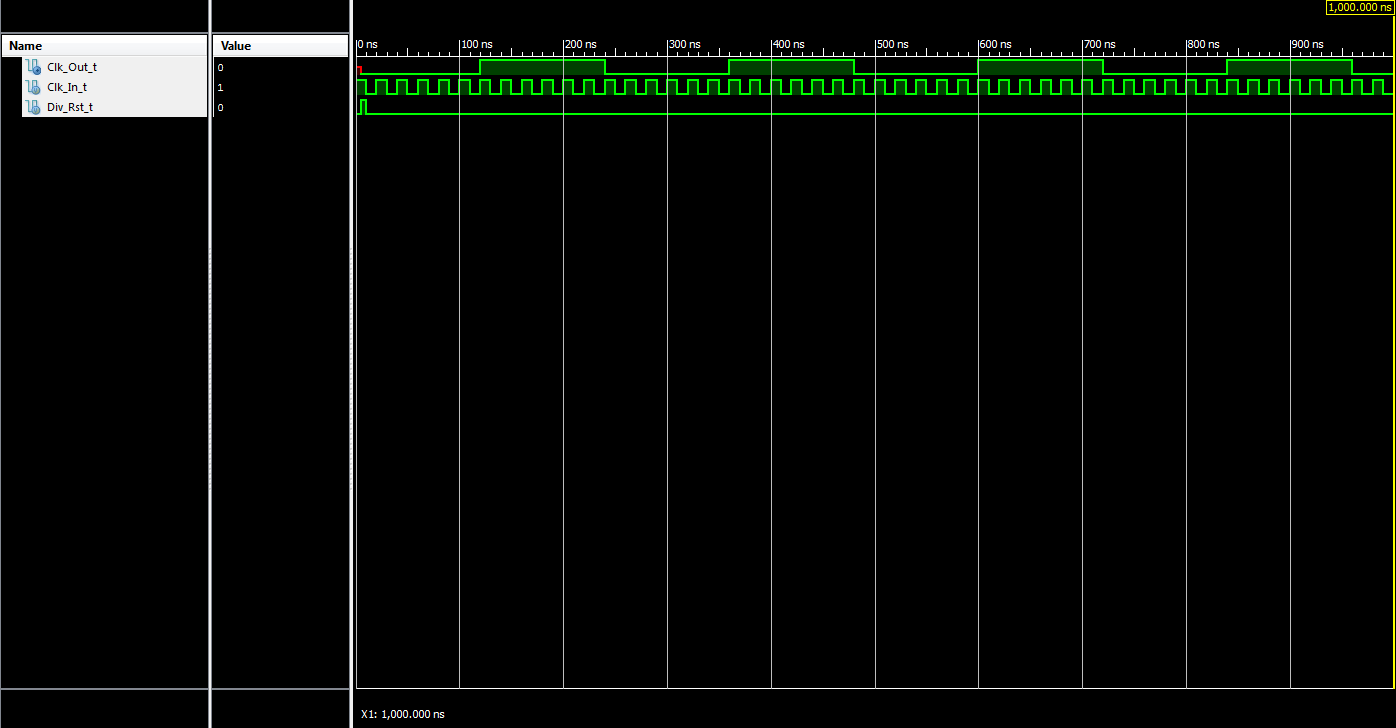
\includegraphics[scale=.45]{cd.PNG}
			\end{center}
				\paragraph*{}
				This waveform shows dividing the Sparten3E's 50mHz clock cycle into a 5mHz clock cycle by using a divider of 5.  We did this so we could see the tested behavior in the sim.  To achieve 1mHz we will use a divider of 25 million in the actual implementation.
		
			\begin{center}
				\textbf{2x1 Multiplexor Simulation}
				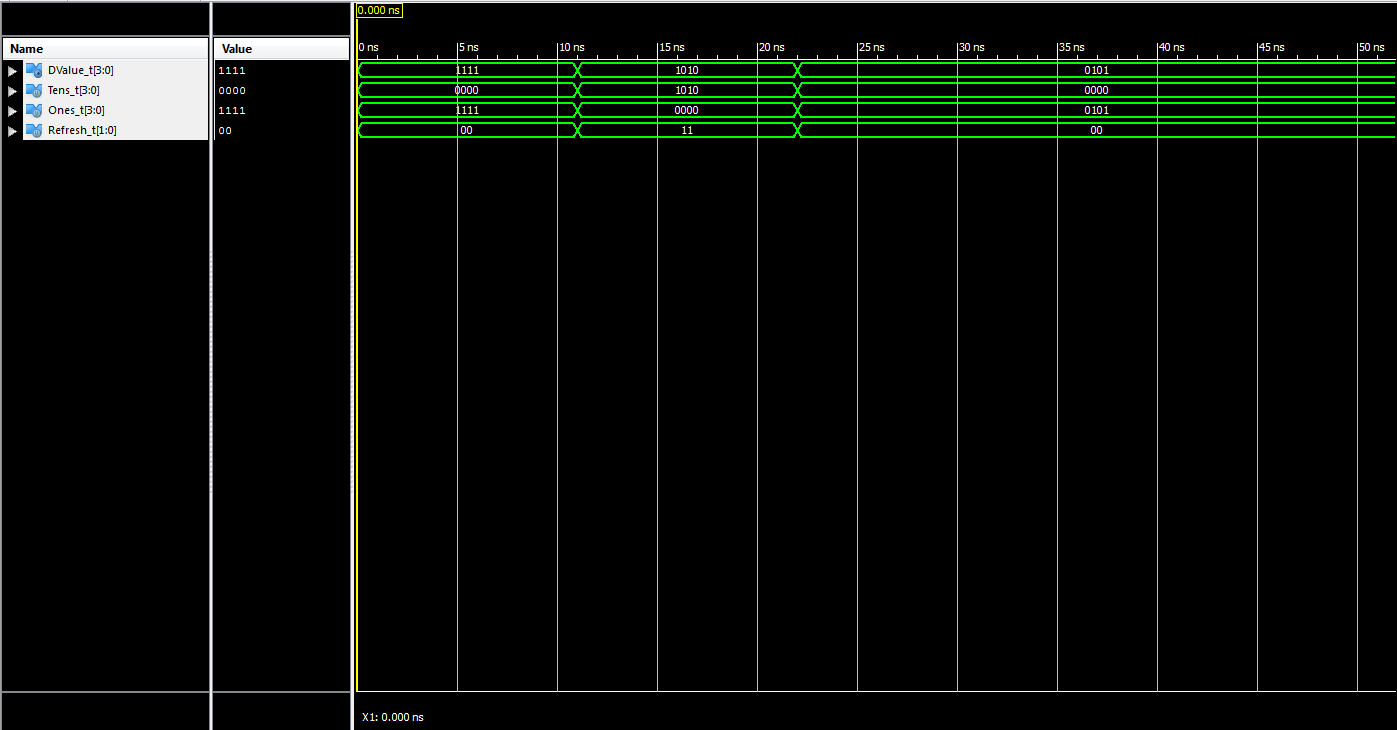
\includegraphics[scale=.45]{mux.PNG}
			\end{center}
				\paragraph*{}
				This waveform shows how the multiplexor will output the tens value of the ones value based on the state of refesh.  The values used are not realistic but rather just used to shows that the logic of the module works.
				
			\begin{center}
				\textbf{Refresh Simulation}
				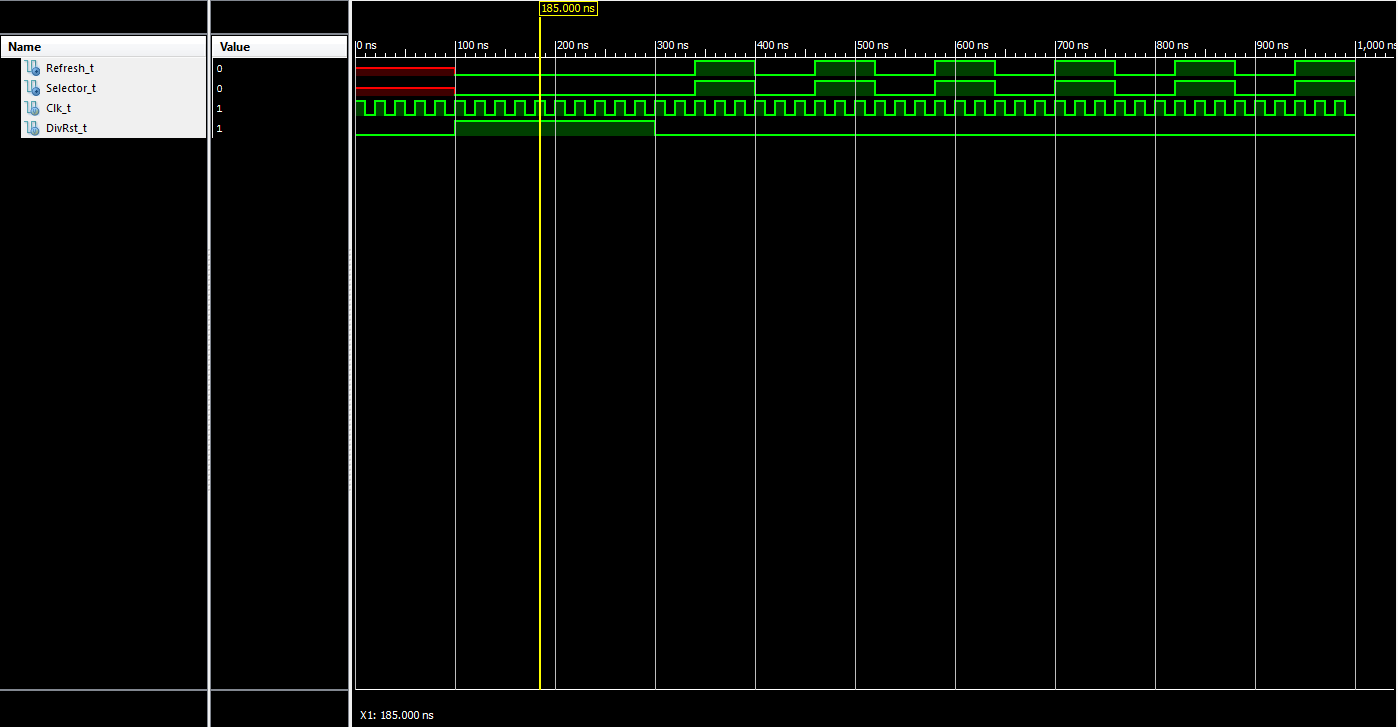
\includegraphics[scale=.45]{re.PNG}
			\end{center}
				\paragraph*{}
				This waveform shows how the value of DivRst and Refresh act on Selector or the value that determines the display digit.  When refresh is high selector is high and the tens digits is refreshed.  When refresh is low the ones digit is refreshed.  Finally when DivRst is high the current state hold until DivRst is low again.
			
			\begin{center}
				\textbf{UpDown Simulation}
				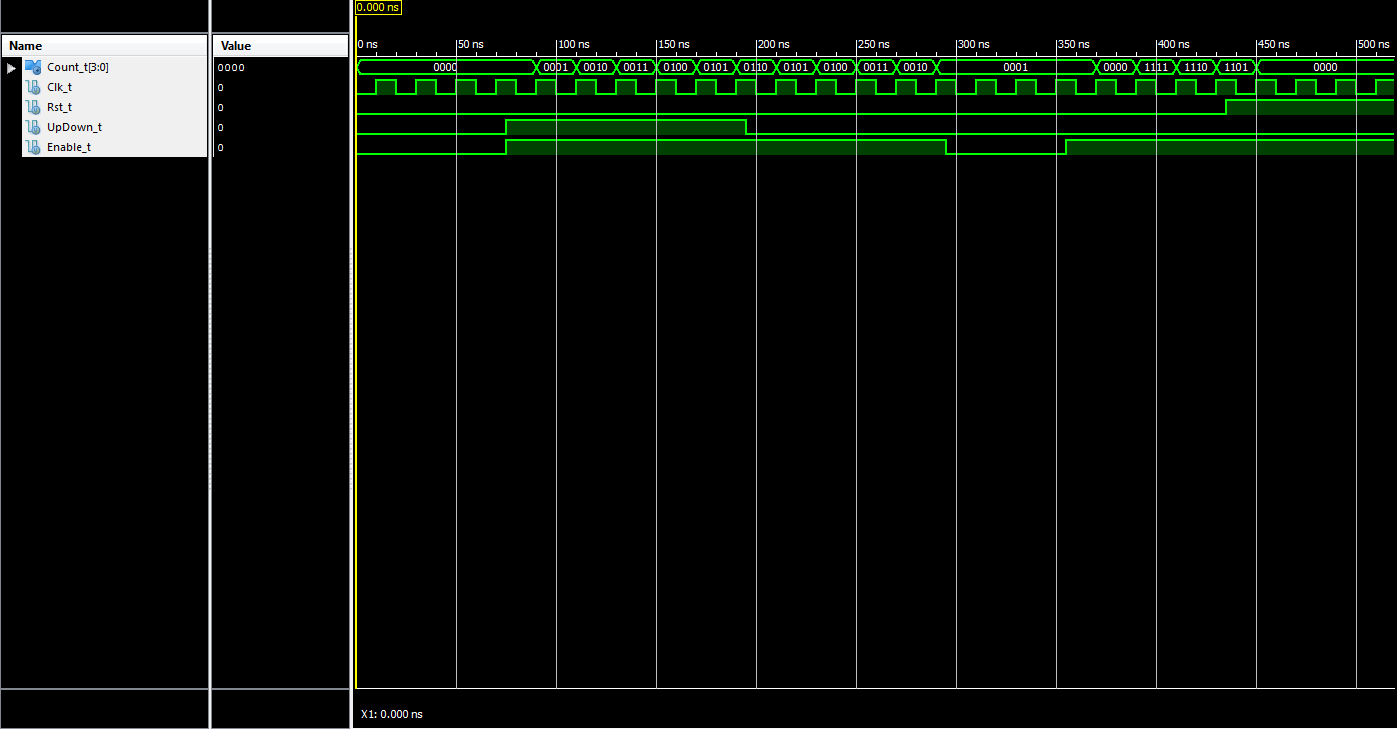
\includegraphics[scale=.45]{cnt.PNG}
			\end{center}
				\paragraph*{}
				This is from a previous lab and show the behavior of UpDown.  When Enable is low or DivRst is high the current state is held until the opposite of each of those values.  If UpDown is high the values are counted up and wrap around.  The opposite is true when UpDown is low.  Finally if reset is high it resturns to the 0 state.
				\newpage

			\begin{center}
				\textbf{Seven Segment Display Simulation}
				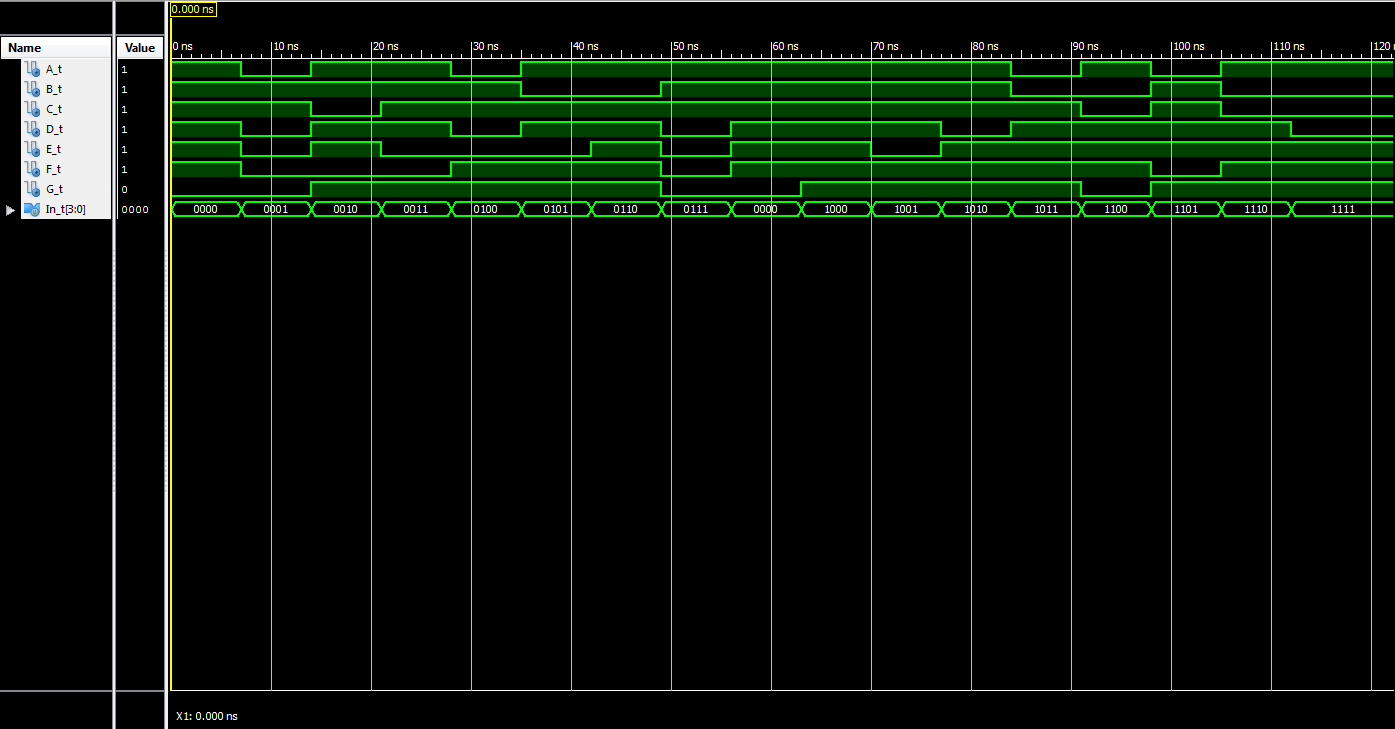
\includegraphics[scale=.45]{seg.PNG}
			\end{center}
				\paragraph*{}
				This waveform shows how the actual value is mapped two the seven segement display.  The value of In is the number that we wish to display and the values of A-G are set high when we want that LED segment on.  We combine these LEDs to display certain numbers adn that is shown in the waveform.

			\begin{center}
				\textbf{Binary To Binary Coded Decimal Simulation}
				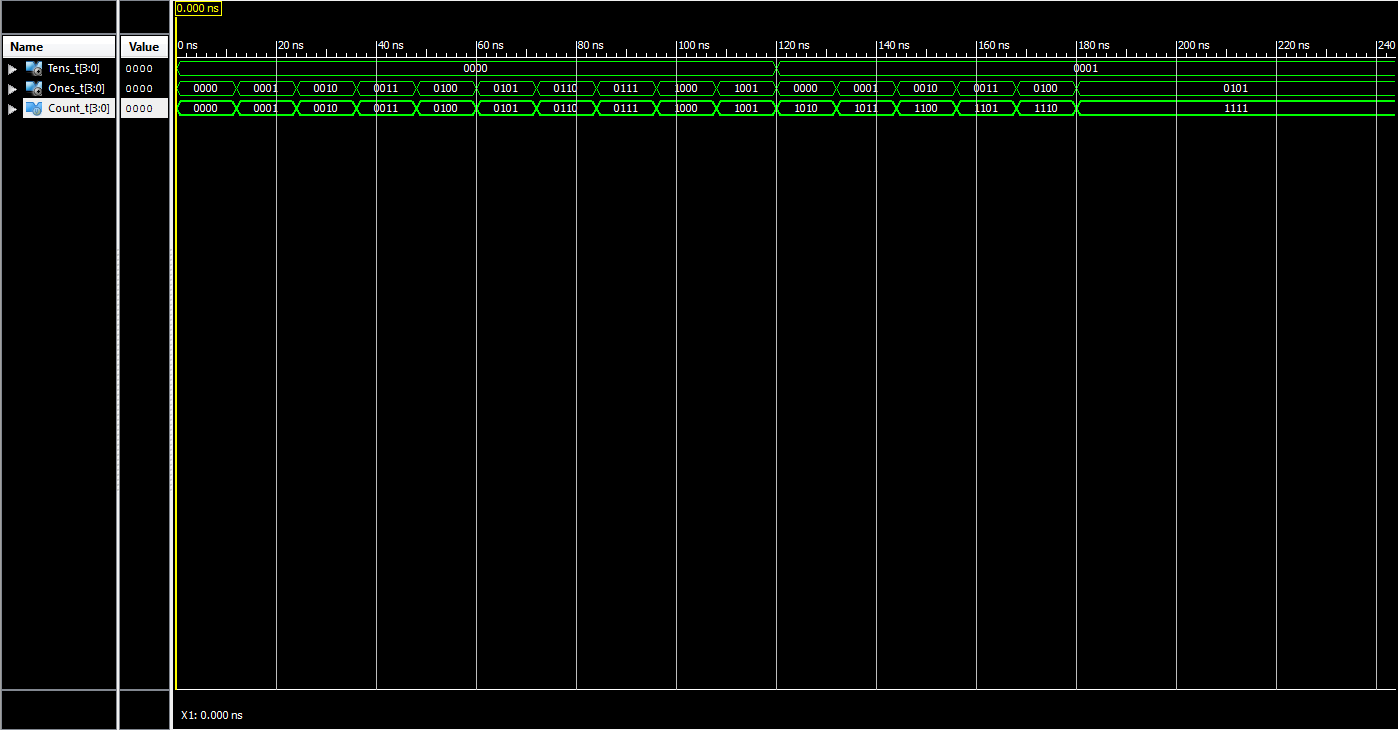
\includegraphics[scale=.45]{b2bcd.PNG}
			\end{center}
				\paragraph*{}
				This waveform simulates the way that binary coded decimal is supposed to work.  The counter is split into two variables or two digits.  When ones counts up to 10 it is reset to 0 and tens is increased to one.  When Ones counts down from 0 tens is decreased to 0 and ones is set to nine.  All other behavior is that same from previous labs counting in Hex.
			
\section*{Significance}
	\paragraph{}
		The introduction of the Binary Coded Decimal and Refresher features add a great deal of human readability and simplicity to the physical implementation, and overall improve the UpDown design. Binary Coded Decimal translation is a very useful technique that is used across several areas of computer systems when displaying a number is needed. The same goes for the display driver that we implemented. Whether 7-segment displays or other LED screens, knowing the digital design behind it is very useful and important.

\section*{Comments/Suggestions}
	\paragraph{}
		The lab was a nice, natural extension of UpDown. The lab demo requirements seemed clear up until the actual demo, when we had one large testbench file, according to the ``Demo the overall module testbench waveform...'' instruction, and we were actually supposed to have separate testbenches for each module. This turned out to not be a problem since we had just enough time to implement them, except for the Refresher module, which was working great on the board, but not on the testbench, and it was not explicitly mentioned in the Lab Demo requirements, as said before.
		
\end{document}


